The rising of quantum computing in the last few year became the attention of researchers to schemes that uses cryptography primitives different from discrete logarithm and number factorization. As mentioned before in Chapter \ref{ch:intro}, code-based cryptosystems are those who uses fundamental aspects of coding theory to add redundancy to a plain text, to intentionally add errors and recovery the plain text. 

In this Chapter, we will explain the first cryptosystem based on coding theory. Furthermore, we will show an Round One code-based submission to the NIST standardization process, the BIGQUAKE, and we show the timing side-channel attack performed in the reference implementation of the scheme.

\section{McEliece Cryptosystem}
Robert J. McEliece proposes in 1978 the first cryptosystem based on coding theory, the McEliece cryptosystem was based on the Goppa codes and uses them to achieve three main algorithms, i. e. Key Generation, Encryption and Decryption \cite{mceliece1978public}. The Figure \ref{fig:code-idea} shows the main of the McEliece Cryptosystem and most of schemes based in coding theory. Given a plaintext and a public encoding function, anyone can generate a codeword and intentionally add some errors to obtain a ciphertext. From this ciphertext, only who has knowledge from the code structure are able to perform a decoding function and recover the plaintext.


\begin{figure}
    \centering
    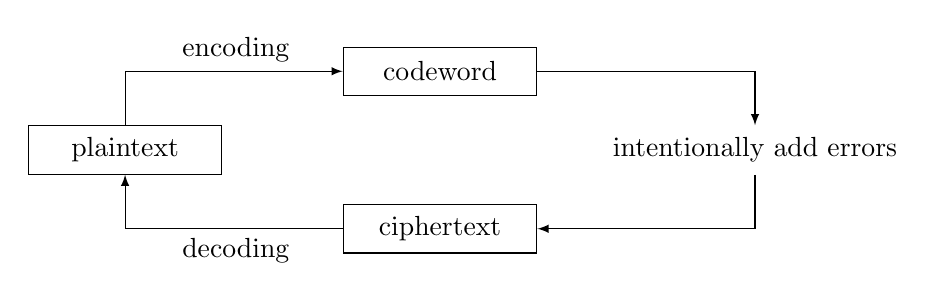
\begin{tikzpicture}
    \node[draw, minimum width=70pt, minimum height=17.5pt] (plain1) at (0, -1) {plaintext};
    \node[draw, minimum width=70pt, minimum height=17.5pt] (ciphertext) at (4, -2) {ciphertext};
    \node[draw, minimum width=70pt, minimum height=17.5pt] (codeword) at (4, 0) {codeword};
    \node[minimum width=70pt, minimum height=17.5pt] (adderror) at (8, -1) {intentionally add errors};
    \draw[-latex] (plain1) |- node[above, xshift=40pt]{encoding} (codeword);
    \draw[-latex] (codeword) -| (adderror);
    \draw[-latex] (adderror) |- (ciphertext);
    \draw[-latex] (ciphertext) -| node[below, xshift=40pt]{decoding} (plain1);
    \end{tikzpicture}
    \label{fig:code-idea}
    \fonte{the author.}
    \caption{Code-based cryptography main idea.}
\end{figure}

Based on two well know problems, the security of McEliece has remained stable. The first assumption was the hardness of generic decoding and it is NP-complete and is also consider hard on average. The second assumption that regards the security of the McEliece scheme was the indistinguishability of the code. This second assumption is not old as the first one, but it relates to old problems of algebraic coding theory and its consider valid for Goppa Codes, as the original proposal. 

The original parameters were designed for $2^{64}$ security bits, but it easily scales up to provided an ample security margin against attackers. Furthermore, the McEliece Cryptosystem suffer many structural attacks, and until today the original proposal remains consider secure. It is important note that many of the attacks are based on the same strategy, the information set-decoding, this kind of attack does not affect schemes based on Goppa codes, however, many others families of codes suffer several drawbacks with this attack. 

As proposed on NIST standardization process by \cite{bernstein2017classic, bigquake, others} the McEliece cryptosystem, using binary Goppa codes, could be applied to concept an KEM, as defined in Chapter \ref{ch:math}. Based on this fact, we can generalized the cryptosystem in three algorithms, the Key generation and Encryption will be explained in Section \ref{sub:mc-def} and Decryption in Section \ref{sub:mc-dec}.

\subsection{Definitions}
\label{sub:mc-def}
Code definitions

Key generation algorithm

Encryption algorithm

\subsection{Decryption}
\label{sub:mc-dec}
Decryption algorithm

Patterson algorithm

Root finding method


\section{BIGQUAKE}
\subsection{Submission overview}
\subsection{Timing side-channel attack}